\documentclass{article}
\usepackage[utf8]{inputenc}
\usepackage{graphicx}
	\DeclareGraphicsExtensions{.png, .jpeg}
\usepackage[top=1in, bottom=1in, left=1in, right=1in]{geometry}

\title{Autonomoboro \\ Lab05: Line Following}
\author{Bandith Phommounivong, Terence Henriod}
\date{\today}

\begin{document}

\maketitle

\begin{abstract}
A dicussion of a robot designed to follow a line and then return home when called for.
\end{abstract}

\newpage

\section{Robot Design}
	\subsection{Hardware Configuration}

Some other text.

	\begin{figure}[h!]
	\centering
	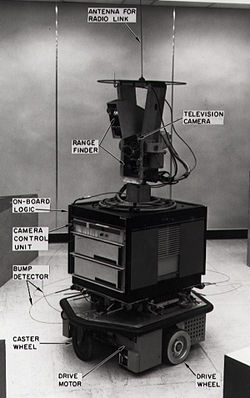
\includegraphics[width = 0.4\textwidth]{shakey}
	\caption{A bad robot.}
	\label{fig:bad_robot}
	\end{figure}

	\subsection{Software Design}

\section{Implementation Problems and Their Solutions}

\section{Unsolved Problems}

\end{document}
